\section{Hardware description}

% Describe the hardware, highlighting the customization rather than the steps of the procedure. Highlight how it differs/which advantage it offers over pre-existing methods. For example, how could this hardware: be compared to other hardware in terms of cost or ease of use, be used in the development of further designs in a particular area, and so on.

% > Add 3-5 bulleted points to broadly explain to other researchers how the hardware could be potentially useful to them, for either standard or novel laboratory tasks, inside or outside of the original user community.

\begin{figure}
	%\begin{adjustwidth}{-\extralength}{0cm}
		%\centering
		\begin{minipage}[b]{11cm}
			\subcaptionbox{}
			{\includesvg[height=5.5cm,inkscapelatex=false]{figs/SystemDesign1}}
		\end{minipage}
		\begin{minipage}[b]{4cm}
			\subcaptionbox{}
			{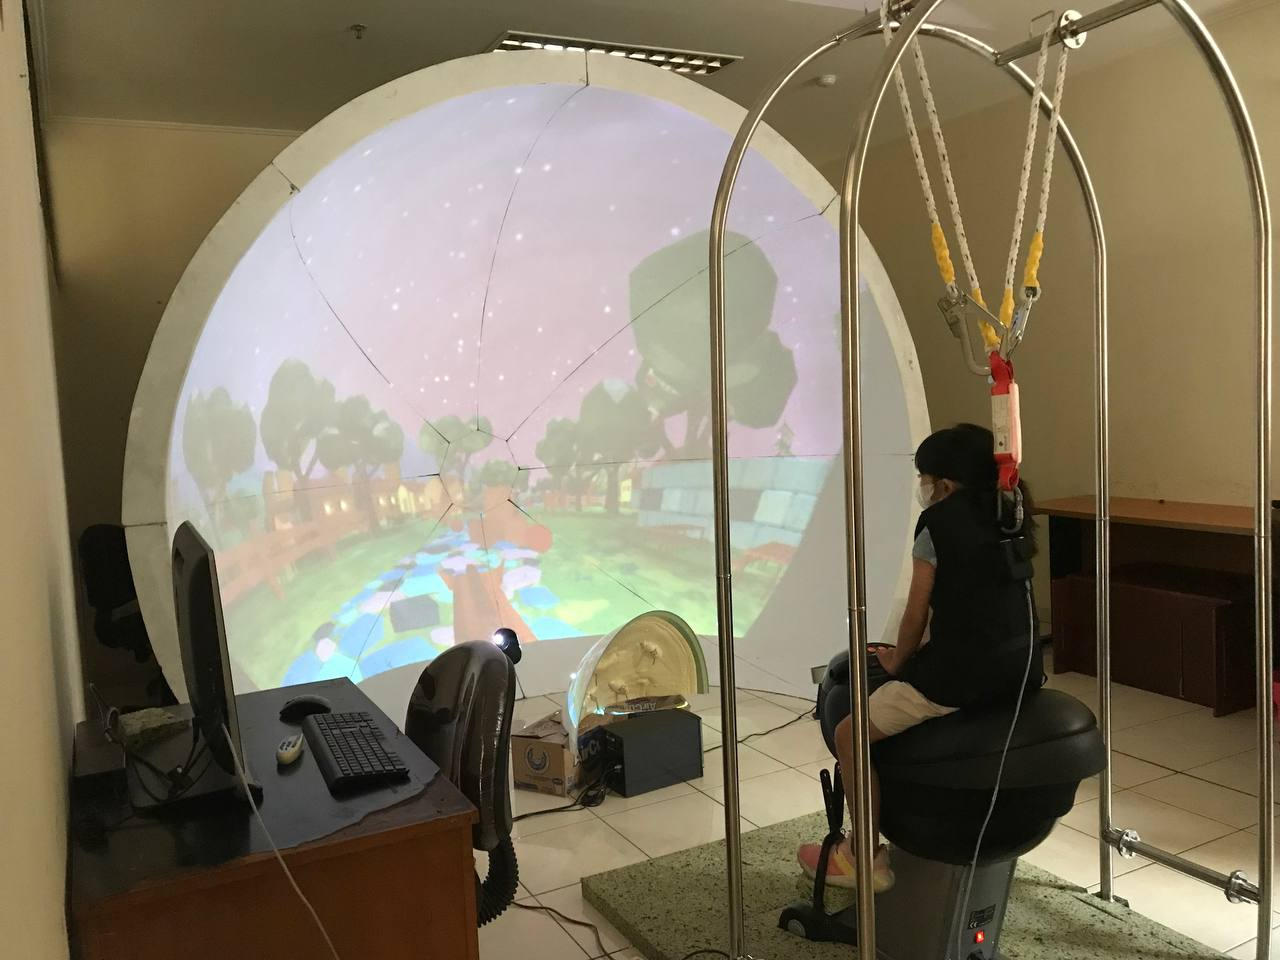
\includegraphics[height=4.5cm]{figs/FotoSystem}}%
		\end{minipage}%
		%\end{adjustwidth}
		\caption
		{%
			(a) System design diagram. (b) Design implementation in use.
			\label{Fig1Horse}%
		}%
\end{figure}

Describe the hardware, highlighting the customization rather than the steps of the procedure. Highlight how it differs/which advantage it offers over pre-existing methods. For example, how could this hardware: be compared to other hardware in terms of cost or ease of use, be used in the development of further designs in a particular area, and so on. \linebreak \linebreak Add 3-5 bulleted points to broadly explain to other researchers how the hardware could be potentially useful to them, for either standard or novel laboratory tasks, inside or outside of the original user community.
\begin{itemize}[noitemsep, topsep=-2pt]
\item Use of the hardware 1
\item Use of the hardware 2
\item Use of the hardware 3
\end{itemize}

\subsection{Dome Design}
As an Immersive Virtual Environment infrastructure, we
build DOME, for several reasons\\

\noindent $D_g$ = eye height in sitting position (cm) for 7-17 years old

\begin{equation}
    F-measure = 2 * \frac{precision * recall}{precision + recall}
    \label{eq4}
\end{equation}

\noindent with:

\noindent $TP$ = True Positive

